\documentclass[12pt]{article}
\usepackage[utf8]{inputenc}
\usepackage[francais]{babel} 
\usepackage[T1]{fontenc}
\usepackage{amsmath}
\usepackage{amsfonts}
\usepackage{amssymb}
\usepackage{graphicx}
\usepackage{listings}
\usepackage{caption}
\usepackage{color}
\usepackage{xcolor}
\usepackage{lineno,amssymb}
\usepackage{array}
\usepackage{fancyhdr}
\usepackage{ifpdf}

\renewcommand{\floatpagefraction}{.999} 
\renewcommand{\textfraction}{.001}
\setcounter{totalnumber}{3} 

\definecolor{dkgreen}{rgb}{0,0.6,0}
\definecolor{gray}{rgb}{0.5,0.5,0.5}
\definecolor{mauve}{rgb}{0.58,0,0.90}

\DeclareCaptionFont{white}{\color{white}}
\DeclareCaptionFormat{listing}{\colorbox{gray}{\parbox{\textwidth}{#1#2#3}}}
\captionsetup[lstlisting]{format=listing,labelfont=white,textfont=white}
\renewcommand{\captionfont}{\small}
\setlength{\captionmargin}{13pt}
\setlength{\belowcaptionskip}{10pt}
\setlength{\abovecaptionskip}{10pt}

%\usepackage[left=2cm,right=2cm,top=2cm,bottom=2cm]{geometry}

\lstset{%
%frame=tRBl,
numbers=left,
numberstyle=\tiny,
frameround=tttt,
basicstyle=\footnotesize,%\sffamily,
captionpos=t,
stringstyle=\ttfamily,
backgroundcolor=\color{gray!5},
rulecolor=\color{black!30},
%inputencoding=utf8,
extendedchars=\true,%
showspaces=false,               % show spaces adding particular underscores
showstringspaces=false,         % underline spaces within strings
showtabs=false,                 % show tabs within strings adding particular underscores
keywordstyle=\color{blue},          % keyword style
commentstyle=\color{dkgreen},       % comment style
stringstyle=\color{mauve},         % string literal style
tabsize=2,
frame=trbl,
frameround=ffff,
xrightmargin=0pt,
%framexbottommargin=5pt,
xleftmargin=0pt,
columns=fullflexible,
basewidth=0.50em,
fontadjust=false,
lineskip=0pt,
xleftmargin=0pt,
framexleftmargin=0pt,
framexrightmargin=0pt,
framexbottommargin=3pt,
framextopmargin=3pt,
%inputencoding=utf8/latin1,%
literate={à}{{\`{a}}}2 {ê}{{\^{e}}}1 {è}{{\`{e}}}1 {ï}{{\¨{i}}}1 {ë}{{\¨{e}}}1 {î}{{\^{i}}}1 {é}{{\'{e}}}1 {ç}{{\c{c}}}1 {Ç}{{\c{C}}}1%
}

\ifpdf%
\usepackage[%
  pdfauthor={Alain Plantec},%
  pdfsubject={Méta-modélisation, vérification et validation : une approche outillées par l'orienté données},%
  pdftitle={Méta-modélisation, vérification et validation : une approche outillées par l'orienté données},%
  pdfkeywords={},%
  pdfstartview=FitH,%
  bookmarks=true,%
  bookmarksopen=true,%
  breaklinks=true,%
  colorlinks=true,%
  linkcolor=blue,anchorcolor=blue,%
  citecolor=blue,filecolor=blue,%
  menucolor=blue,%
  urlcolor=blue]{hyperref}
\else
\usepackage[%
  breaklinks=true,%
  colorlinks=true,%
  linkcolor=blue,anchorcolor=blue,%
  citecolor=blue,filecolor=blue,%
  menucolor=blue,%
  urlcolor=blue]{hyperref}
\fi

\lstdefinelanguage{express}
{keywords={ABS,ABSTRACT,ACOS,AGGREGATE,ALIAS,AND,ANDOR,ARRAY,
	AS,ASIN,ATAN,BAG,BEGIN,BINARY,BLENGTH,BOOLEAN,BY,
	CASE,CONST_E,CONSTANT,CONTEXT,COS,DERIVE,DIV,ELSE,
	END,END_ALIAS,END_CASE,END_CONSTANT,END_CONTEXT,END_ENTITY,
	END_FUNCTION,END_IF,END_LOCAL,END_MODEL,END_PROCEDURE,END_REPEAT,
	END_RULE,END_SCHEMA,END_TYPE,ENTITY,ENUMERATION,ESCAPE,EXISTS,
	EXP,FIXED,FOR,FORMAT,FROM,FUNCTION,GENERIC,HIBOUND,HIINDEX,
	IF,IN,INSERT,INTEGER,INVERSE,LENGTH,LIKE,LIST,LOBOUND,LOCAL,
	LOG,LOG10,LOG2,LOGICAL,LOINDEX,META, MOD,MODEL,NOT,NUMBER,NVL,
	ODD,OF,ONEOF,OPTIONAL,OR,OTHERWISE,PI,PROCEDURE,QUERY,REAL,
	REFERENCE,REMOVE,REPEAT,RETURN,ROLESOF,RULE,SCHEMA,SELECT,
	SELF,SET,SIN,SIZEOF,SKIP,SQRT,STRING,SUBTYPE,SUPERTYPE,
	TAN,THEN,TO,TYPE,TYPEOF,UNIQUE,UNTIL,USE,USEDIN,VALUE,
	VALUE_IN,VALUE_UNIQUE,VAR,WHERE,WHILE,XOR},
sensitive=f,
morestring=[d]",
morestring=[d]',
morecomment=[s]{(*}{*)},
morecomment=[l]--
}[keywords,comments,strings]

\author{Alain Plantec}

\title{Génération de code et interopérabilité}
\begin{document}
\thispagestyle{empty}
\maketitle

\tableofcontents
\pagebreak
\textit{minispec} est un langage de modélisation de données. Il permet la spécification d'entités, comprenant un ensemble d'attributs typés. Le projet consiste à mettre en œuvre un noyau logiciel utilisant \textit{minispec} comme langage pivot pour de la génération de code et pour la mise en œuvre de langages spécialisés. 

Le projet se constitue d'une suite d'exercices. Chaque exercice ajoute un besoin supplémentaire. L'idée est de faire évoluer progressivement votre mise en œuvre pour répondre aux nouveaux besoins. La résolution  d'un exercice peut donc nécessiter de revoir la façon dont vous avez traité les exercices précédents. 

\section{Une version minimale pour démarrer}
Vous allez développer un premier méta-modèle pour une version minimale du langage \textit{minispec} et un outil de génération de code vers Java. 

Le travail à éffectuer consiste à développer une première version simple d'un générateur de code vers Java.

La première version de \textit{minispec} intègre uniquement la déclaration d'entités avec des attributs de type primitif (String, Integer...). La figure~\ref{fig:exemple-minispec1} montre un exemple simple de specification avec \textit{minispec}. Une telle spécification peut servir de source à un générateur de code vers un langage de programmation. Par exemple, il est possible de générer le code \textit{Java} de la figure~\ref{fig:code-java-genere1}

\begin{figure}
\begin{lstlisting}[language=express]
entity Satellite ;
  nom: String ;
  id:Integer ;
end_entity ;
\end{lstlisting}
\caption{Un exemple de specification avec \textit{minispec}}
\label{fig:exemple-minispec1}
\end{figure} 


\begin{figure}
\begin{lstlisting}[language=java]
public class Satellite {
  String nom ;
  Integer id ;
  public Satellite() { }
  public String getNom() { return nom ; }
  public void setNom(String nom) { this.nom = nom ; }
}
\end{lstlisting}
\caption{Le code Java pouvant être généré à partir de notre exemple}
\label{fig:code-java-genere1}
\end{figure} 

Comme le montre la figure~\ref{fig:generation-code-1}, pour générer ce code, les deux étapes suivantes sont mises en oeuvre :
\begin{enumerate}
	\item il faut analyser le code \textit{minispec} et construire une représentation mémoire de ce code sous la forme d'un graphe d'objets ;
	\item il faut parcourir le graphe d'objet pour produire une chaines de caractères contenant le code \textit{Java}.
\end{enumerate}

\begin{figure}
\begin{center}
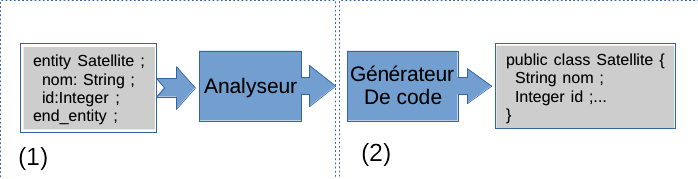
\includegraphics[scale=0.5]{generation-code-1.png}
\end{center}
\caption{Mise en oeuvre classique d'une génération de code}
\label{fig:generation-code-1}
\end{figure} 

Pour l'analyse du code \textit{minispec}, il faut disposer de la grammaire du langage utilisé en entrée et développer l'analyseur pour le langage. Pour une syntaxe textuelle telle que celle utilisée dans l'exemple, on peut utiliser un générateur de compilateur tel que Lex/Yacc. La création de la représentation interne (graphe d'objets) est alors programmée dans les actions sémantiques.

\begin{figure}
\begin{center}
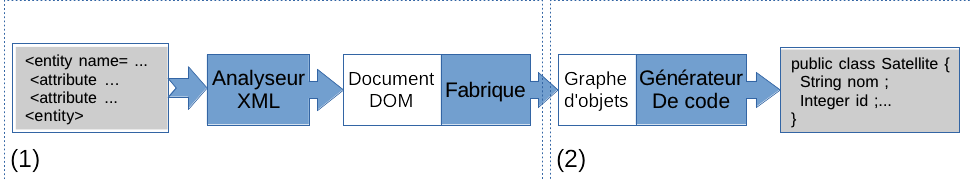
\includegraphics[scale=0.5]{generation-code-2.png}
\end{center}
\caption{Mise en oeuvre d'une génération de code en utilisant XML pour la représentation source}
\label{fig:generation-code-2}
\end{figure} 

Une seconde solution plus simple consiste à utiliser une syntaxe XML pour représenter le code \textit{minispec}. Cette solution permet de tester la génération de code sans avoir à programmer un analyseur pour la syntaxe textuelle spécifique. Cette solution est montrée par la figure~\ref{fig:generation-code-2}. En entrée, la première étape lit un fichier XML qui représente une spécification en minispec. Par exemple, le code XML de la figure~\ref{fig:exemple-minispec-XML1} peut être utilisé comme l'équivalent de notre exemple de modèle avec l'entité Satellite :
\begin{figure}
\begin{lstlisting}[language=XML]
<entity name="Satellite">
  <attribute name="nom" type="String"/>
  <attribute name="id" type="Integer"/>
</entity>
\end{lstlisting}
\caption{Specification de notre exemple de modèle en XML}
\label{fig:exemple-minispec-XML1}
\end{figure} 

L'analyseur XML produit un document DOM. Pour l'étape 2, une fabrique exploite le document DOM pour produire le graphe d'objets de la représentation interne. La représentation interne est parcourue à l'aide d'un visiteur qui produit le code Java.

Pour générer le code \textit{Java}, on utilise une représentation interne issue du modèle XML en entrée. Cette représentation interne est un ensemble d'instances constituant un graphe d'objets. Les classes de ces objets sont décrits par un modèle particulier : le méta-modèle de \textit{minispec}. Ces classes peuvent être par ailleurs décrite à l'aide d'un modèle UML constituant ainsi une autre représentation du méta-modèle de \textit{minispec}. La représentation interne est dite conforme aux méta-modèles. Le modèle UML d'un exemple de méta-modèle pour \textit{minispec} est montré dans la figure~\ref{fig:meta-modele-UML1}. 
\begin{figure}
\begin{center}
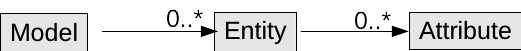
\includegraphics[scale=0.5]{modeleUML1.png}
\end{center}
\caption{Un métamodèle de minispec présenté en UML}
\label{fig:meta-modele-UML1}
\end{figure} 

La figure~\ref{fig:meta-model-java1} montre le squelette des classes Java correspondant au modèle UML~\ref{fig:meta-modele-UML1}.

\begin{figure}
\begin{center}
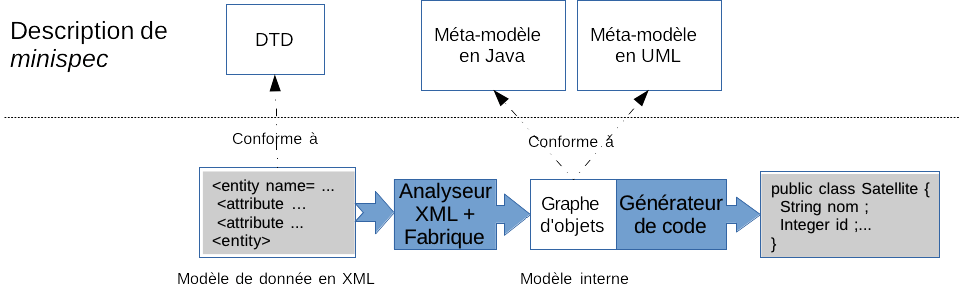
\includegraphics[scale=0.5]{generation-code-3.png}
\end{center}
\caption{Schéma de la chaine d'outils avec les méta-modèles}
\label{fig:generation-code-3}
\end{figure} 

\begin{figure}
\begin{lstlisting}[language=java]
class Model {
  String nom ;
  List<Entity> entities;
}
class Entity {
  String nom ;
  List<Attribute> attributes;
}
class Attribute {
  String nom ;
  String type;
}
\end{lstlisting}
\caption{Un métamodèle de minispec présenté en Java}
\label{fig:meta-model-java1}
\end{figure} 

\section{Associations unidirectionnelles entre entités}
\subsection{Association simple}
Avec \textit{minispec}, une association unaire d'une entité A avec une entité B est modélisée à l'aide d'un attribut de l'éntité A dont le type est B. Cette association spécifie que toute instance de l'entité A est associé avec une instance de l'entité B.
\begin{figure}
\begin{lstlisting}[language=express]
entity Satellite ;
  nom: String ;
  id:Integer ;
  parent : Flotte;
end_entity ;
entity Flotte;
end_entity;
\end{lstlisting}
\caption{Un exemple de specification avec une association simple entre deux entités}
\label{fig:exemple-minispec2}
\end{figure} 
La figure~\ref{fig:exemple-minispec2} montre une association simple entre l'entité \textit{Satellite} et l'éntité \textit{Flotte}. Cette association est  spécifiée par l'attribut \textit{parent}. Le nom \textit{Flotte} est utilisé comme type de l'attribut parent. La figure~\ref{fig:exemple-minispec-XML2} montre comment représenter cette association en XML. On remarque que le nom \textit{Flotte} est directement utilisé comme valeur de l'attribut \textit{type} pour indiquer le type de l'attribut \textit{parent}.
\begin{figure}
\begin{lstlisting}[language=XML]
<entity name="Satellite">
  <attribute name="nom" type="String"/>
  <attribute name="id" type="Integer"/>
  <attribute name="parent" type="Flotte"/>
</entity>
<entity name="Flotte">
</entity>
\end{lstlisting}
\caption{Specification d'une association simple en XML}
\label{fig:exemple-minispec-XML2}
\end{figure} 




\subsection{Association multiple}
Une association multiple est utilisée pour indiquer une relation d'une instance d'entités avec potentiellement plusieurs autres instances d'entités. Dans la figure~\ref{fig:exemple-minispec3}, l'entité \textit{Flotte} est complétée avec l'attribut \textit{satellites} qui spécifie une collection d'instances de \textit{Satellite}. 
\begin{figure}
\begin{lstlisting}[language=express]
entity Flotte;
  satellites : List of Satellite;
end_entity;
\end{lstlisting}
\caption{Une association multiple entre deux entités}
\label{fig:exemple-minispec3}
\end{figure} 

Il peut être interessant d'indiquer des cardinalités min et max. Par exemple, dans la figure~\ref{fig:exemple-minispec4}, les cardinalités indiquent explicitement qu'une flotte comporte au minimum 1 satellite et au maximum 10. Ces informations peuvent être utilisées pour implanter des controles dans les méthodes permettant de modifier les collections ou générer des tests.
\begin{figure}
\begin{lstlisting}[language=express]
entity Flotte;
  satellites : List [1:10] of Satellite;
end_entity;
entity Satellite;
  panneaux : Array [2] of PanneauSolaire; 
end_entity;
\end{lstlisting}
\caption{Exemples d'associations multiples avec des cardinalités (List) ou une taille fixe (Array)}
\label{fig:exemple-minispec4}
\end{figure}

Le type de collection utilisé peut etre \textit{List}, \textit{Set}, \textit{Bag} ou \textit{Array}. Attention donc aux points suivants:
\begin{itemize}
	\item Le métamodèle doit être adapté pour supporter les collections à plusieurs dimensions et les collections de natures différentes (\textit{List}, \textit{Array}, \textit{Set}, \textit{Bag});
	\item Un tableau (Array) est de taille fixe, les autres collections (List, Set, Bag) peuvent avoir une cardinalité minimale et maximale;	
\end{itemize}

La première version du méta-modèle montrée dans la figure~\ref{fig:meta-model-java1} n'est plus suffisante. Il vous faut l'adapter pour pouvoir stocker les informations concernant les associations multiples avec les cardinalités ou la taille. 

De même, il vous faut déterminer une syntaxe XML adéquate pour spécifier une association multiple.

%\subsection{Association multiple à deux dimensions ou plus}
%Il est courant de vouloir spécifier des associations multiples à plusieurs dimensions. Par exemple, considérons l'exemple de modélisation d'un jeu de bataille navale. Une telle modélisation peut contenir une entité \textit{Grille} comprenant un attribut \textit{cases} correspondant à la matrice de cases du jeux. L'entité Grille est montrée dans la figure~\ref{fig:exemple-minispec5}.
%
%\begin{figure}
%\begin{lstlisting}[language=express]
%entity Grille;
%  cases : Array [25] of Array [25] of Boolean; 
%end_entity;
%\end{lstlisting}
%\caption{Une association multiple à plusieurs dimensions}
%\label{fig:exemple-minispec5}
%\end{figure} 
%
%Attention, pour la spécification XML, utiliser directement le nom d'un type pour le référencer n'est plus possible à cause de la seconde dimension du tableau (type anonyme).

\section{Héritage et Modèle}

\subsection{Introduction de l'héritage}
Une entité peut hériter d'une autre entité. L'héritage est simple, une entité ne peut hériter que d'une seulle autre entité. Un exemple d'héritage est montré par la figure~\ref{fig:exemple-minispec6}. Dans cet exemple, l'entité \textit{Chaise} hérite de \textit{Meuble}. 

Du fait de l'héritage, certaines erreurs d'utilisation de minispec peuvent etre introduites. Les deux erreurs courante sont la circularité (\textit{B} hérite de \textit{A} qui hérite de \textit{B}) et la définition multiple d'attributs (l'entité \textit{A} hérite de \textit{B}, \textit{A} et \textit{B} contiennent toutes les deux un attribut de nom \textit{i}).

Il vous faut donc adapter le méta-modèle et la génération de code pour intégrer la relation d'héritage. Il vous aussi vérifier la spécification avant génération de code pour éviter les dépendances circulaires et les définitions multiples d'attributs.

\begin{figure}
\begin{lstlisting}[language=express]
entity Chaise subtype of (Meuble);
end_entity;
\end{lstlisting}
\caption{Utilisation de l'héritage}
\label{fig:exemple-minispec6}
\end{figure} 

\subsection{Modèle et résolution des dépendances}
Les entités appartiennent à un modèle. Dans minispec, un modèle correspond au package en Java. Un modèle porte donc un nom et permet de regrouper des entités. 

Jusqu'à présent le concept de modèle a été éludé. Or, il est important de pouvoir produire du code valide qu'il n'est pas nécessaire de corriger manuellement après génération de code. En java, les dépendances sont explicitement indiquées via les \textit{imports}. Les imports doivent donc être ajoutés automatiquement par le générateur de code. Pour générer les imports, il faut donc se baser sur les modèles de \textit{minispec}. Cependant, il peut être utile d'introduire un second méta-modèle pour permettre de paramétrer correctement la production des imports. Le schéma de la figure~\ref{fig:generation-code-4} montre la chaine d'outils prenant en compte ce nouveau méta-modèle introduit pour le paramétrage de la génération de code.

\begin{figure}
\begin{center}
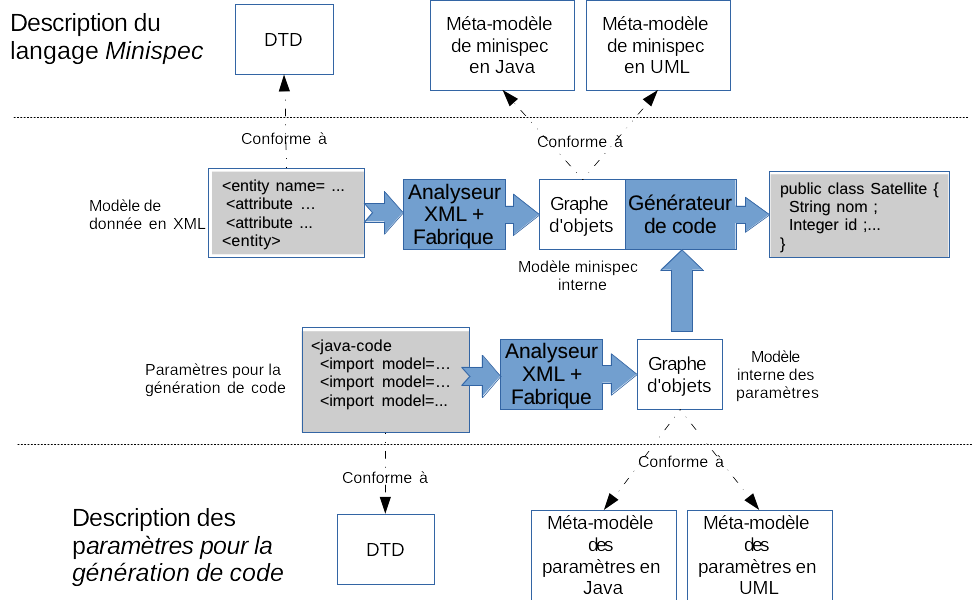
\includegraphics[scale=0.5]{generation-code-4.png}
\end{center}
\caption{Schéma de la chaine d'outils avec les méta-modèles pour minispec et les paramètres de génération de code}
\label{fig:generation-code-4}
\end{figure} 

Le méta-modèle et la syntaxe XML pour le paramétrage doivent donc être ajoutés. Dans cette version et pour cet exercice, le contenu du paramétrage permet essentiellement d'établir le lien entre un modèle minispec et un package Java et d'indiquer le lien entre des types primitifs et leur équivalent en Java. La figure\ref{fig:exemple-parametrage-XML1} montre un exemple de paramétrage.  

\begin{figure}
\begin{lstlisting}[language=XML]
<java-code>
  <model name="Meuble" package="m2tiil.meuble"/>
  <model name="Bataille" package="m2tiil.batailleNavale"/>
  <primitive name="String" type="String"/>
  <primitive name="Integer" type="Integer"/>
  <primitive name="List" type="ArrayList" package="Java.util.ArrayList"/>
  <primitive name="Array" type="Array" package="m2tiil.Array"/>
  <primitive name="Set" type="HashSet" package="Java.util.HashSet"/>
  <primitive name="Bag" type="Bag" package="m2tiil.Bag"/>
</java-code>
\end{lstlisting}
\caption{Exemple de paramétrage en XML}
\label{fig:exemple-parametrage-XML1}
\end{figure} 

Un outil supplémentaire de gestion des dépendances entre modèles doit aussi être mise en oeuvre. Cet outil doit permettre de récupérer et d'ajouter à un package java généré tous les imports nécessaires à sa compilation. Cet outil s'appuie sur un arbre de dépendances entre modèles construit avant génération de code et sur les paramètres de génération de code qui permettent d'ajouter les imports necessaires.

\section{Valeurs initiales des attributs}
Jusqu'à présent, le générateur de code que vous avez programmé n'a pas tenu compte des valeurs initiales des attributs des entités et en conséquence, celle des variables d'instances des classes crées. Les valeurs initiales sont donc celle par défaut en java. 

Cependant, il peut être très utile de pouvoir indiquer des valeurs initiales. La figure~\ref{fig:exemple-minispec7} montre l'exemple de l'entité \textit{Bateau} avec des valeurs initiales. Une valeur initiale est une expression qui peut être une valeur primitive  (comme pour l'attribut \textit{valide}) ou bien l'appel d'une fonction ou d'un constructeur (comme pour les attributs \textit{position} et \textit{id}).
\begin{figure}
\begin{lstlisting}[language=express]
entity Bateau;
  position : Point := Point(0,0);
  nom : String;
  id : Integer := nextId();
  valide : Boolean := false;
end_entity;
\end{lstlisting}
\caption{Spécification de valeurs initiales avec minispec}
\label{fig:exemple-minispec7}
\end{figure} 

Pour tenir compte des valeurs initiales, il vous faut modifier le méta-modèle de minispec, le format XML utilisé pour spécifier des modèles et enfin le générateur de code.

\section{Lot d'instances}
Un lot d'instances est un objet qui gère un ensemble d'instances d'un ou plusieurs modèles. Physiquement, il est représenté par un fichier XLM. En mémoire, un lot comprend les instances et les modèles comprenant les entités dont les instances sont conformes. La figure~\ref{fig:repository-UML1}  montre le modèle d'un lot d'instances spécifié comme un \textit{Repository}.

\begin{figure}
\begin{center}
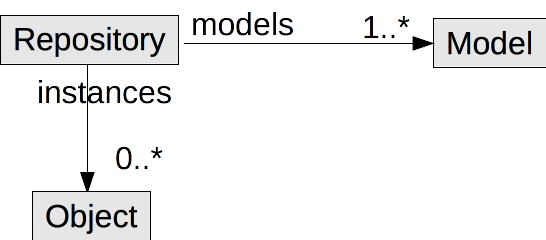
\includegraphics[scale=0.5]{repositoryUML1.png}
\end{center}
\caption{Modélisation d'un lot d'instances en UML}
\label{fig:repository-UML1}
\end{figure}

Les trois fonctions principales d'un lot d'instances sont l'enregistrement, la sérialisation et la matérialisation des instances :
\begin{itemize}
\item L'enregistrement d'une instance consiste à l'intégrer au lot d'instance. 
\item La sérialisation consiste à produire un fichier (par exemple XML) à partir de toutes les instances enregistrées dans un lot d'instances. 
\item La matérialisation consiste à lire un fichier et à reconstituer les instances et les enregistrer dans le lot d'instances.
\end{itemize}

Par exemple, considérons le modèle de la flotte de satellite de la figure~\ref{fig:exemple-minispec8}. Un lot d'instances pour ce modèle contient des instances de l'entité \textit{Flotte} et de l'entité \textit{Satellite}. Un résultat possible de la sérialisation d'un tel lot d'instances est montré par la figure~\ref{fig:exemple-serialisation-XML}. Dans cet exemple, on met en oeuvre les références à l'aide d'identifiants (attribut \textit{id}).

\begin{figure}
\begin{lstlisting}[language=express]
entity Flotte;
  satellites : List [1:10] of Satellite;
end_entity;
entity Satellite;
end_entity;
\end{lstlisting}
\caption{Exemple de modèle simple}
\label{fig:exemple-minispec8}
\end{figure}

\begin{figure}
\begin{lstlisting}[language=XML]
<Satellite id="#1">
</Satellite>
<Satellite id="#2">
</Satellite>
<Satellite id="#3">
</Satellite>
<Flotte satellites="(#1 #2 #3)">
</Flotte>
\end{lstlisting}
\caption{Un exemple de sérialisation}
\label{fig:exemple-serialisation-XML}
\end{figure} 

Vous devez donc modifier votre générateur de code Java pour générer automatiquement un \textit{Repository} spécifique à un ou plusieurs modèles. Le nom du repository peut etre donné par le paramétrage du générateur de code mis en oeuvre précédemment. Les fonctions de sérialisation et de matérialisation du \textit{Repository} sont aussi générées automatiquement. 

La mise en oeuvre du Repository généré peut hériter d'une classe abstraite, par exemple AbstractRepository qui met en oeuvre une partie des fonctions de façon générique. D'autre part, les fonctions de sérialisation et de matérialisation sont basées sur la description des entités présentes dans les modèles associés au lot d'instances.

\section{Rebouclage}
A ce stade de la mise en oeuvre de minispec, on peut remarquer qu'une partie ce qu'on a mis en oeuvre consiste en du code que l'on sait générer à partir d'un modèle minispec:
\begin{itemize}
	\item la définition d'une entité permet de générer la classe avec les accesseurs en lecture et écriture,
	\item le lot d'instance généré permet la sérialisation et la matérialisation à partir de XML.
\end{itemize}

Nous pouvons donc utiliser notre chaine d'outils pour \textit{minispec} lui même en spécifiant le métamodèle de \textit{minispec} avec \textit{minispec}. La figure~\ref{fig:minispec-en-minispec} montre une ébauche de méta-modèle simplifié de \textit{minispec} exprimé avec \textit{minispec}. Ce métamodele peut être exprimé à l'aide de notre format XML et donc être utilisé par notre chaine d'outils pour générer du code java. Or il se trouve que le code java généré peut constituer une partie de la mise en oeuvre de nos outils pour \textit{minispec}...

A vous donc de définir votre métamodèle en vous étant fidèle à votre mise en oeuvre de \textit{minispec} et de générer et utiliser le code java généré pour mettre en oeuvre votre propre chaine d'outils.

\begin{figure}
\begin{lstlisting}[language=express]
model Minispec;
	entity NamedElement;
		name : String;
	end_entity;
	entity ModelDesc subtype of (NamedElement);
  	entities : List of EntityDesc;
	end_entity;
	entity EntityDesc subtype of (NamedElement);
  	attributes : List of AttributeDesc;
	end_entity;
	entity AttributeDesc subtype of (NamedElement);
		domain : TypeDefinition;
		defaultValue : String;
	end_entity;
	entity TypeDefinition;
	end_entity;
	entity EntityType subtype of (TypeDefinition);
		referenced : String;
	end_entity;
	entity CollectionType subtype of (TypeDefinition);
		...
	end_entity;
	...
end_model;

\end{lstlisting}
\caption{Ebauche de métamodèle de minispec en minispec}
\label{fig:minispec-en-minispec}
\end{figure}





\end{document}